%******************************************************************************%
%                                                                              %
%                  sample.tex for LaTeX                                        %
%                  Created on : Tue Mar 10 13:27:28 2015                       %
%                  Made by : David "Thor" GIRON <thor@42.fr>                   %
%                                                                              %
%******************************************************************************%

\documentclass{42}
\graphicspath{{images/}}

%******************************************************************************%
%                                                                              %
%                                  Prologue                                    %
%                                                                              %
%******************************************************************************%
\begin{document}



                           \title{ft\_hangouts}
                          \subtitle{Le Grand Ambassadeur}
                        \member{Pierre-Elie Kesslassy}{pkesslas@student.42.fr}

\summary {
  Le but de ce projet est de vous familiariser avec le syst\`eme Android en
  r\'ealisant une application de gestion de contacts.
}

\maketitle

\tableofcontents


%******************************************************************************%
%                                                                              %
%                                  Préambule                                   %
%                                                                              %
%******************************************************************************%
\chapter{Préambule}

	\begin{center}
	Pas de neige sur le mont Fuji,\\
	ni de fleurs dans les cerisiers,\\
	pas de gazon dans mes plates-bandes,\\
	son règne est minéral.\\
	\vspace{2mm}
	Magique est le liquide,\\
	magique est la source,\\
	magique est le cristal,\\
	magique est le jardin.\\
	\vspace{2mm}
	Le jardinier magicien\\
	cristal, cristal, cristal oh cristal\\
	ho ho ho ho ho ho ho ho ho ho ho ho ho ho ho ho\\
	hohohohohohohohohohohohohohohohohohohohohohohohohohohohohohohoho\\
	hohohohohohohohohohohohohohohohohohohohohohoho ho ho ho ho\\
	\vspace{2mm}
	cristal, cristal, cristal, cristal\\
	Tu ne peux pas le toucher.\\
	Tu n'es pas prêt, tu peux juste le regarder,\\
	Tes yeux sont prêts, tu peux le supporter.\\
	Ouaaaa\\
	Oh c'est beau, c'est beau, c'est beau\\
	\vspace{2mm}
	Le jardinier magicien\\
	n'a pas besoin d'engrais dans son jardin.\\
	brillant comme les étoiles,\\
	brillant comme une mer d'huile,\\
	brillant comme les dents d'un gros chien.\\
	\vspace{2mm}
	brillant comme les insectes,\\
	brillant comme une saucisse,\\
	brillant comme la peau d'un ado.\\
	\vspace{2mm}
	cristal oh cristal\\
	cristal oh cristal\\
	cristal oh cristal\\
	cristal oh crya ha ha\\
	\end{center}

	Salut C'est Cool - \textit{Le jardinier magicien}
	\href{https://www.youtube.com/watch?v=CoCyOX59bhI}{lien}.

%******************************************************************************%
%                                                                              %
%                                 Introduction                                 %
%                                                                              %
%******************************************************************************%
\chapter{Introduction}

	Pour ce projet, vous devrez r\'ealiser une application Android permettant,
	de cr\'eer un contact et de dialoguer avec par SMS.\\
	
	\vspace{5mm}
	Le but ici est de comprendre comment fonctionne une application android,
	comment Android g\`ere votre application et comment utiliser le SDK.

	\begin{center}
	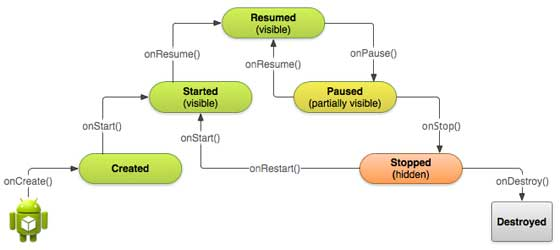
\includegraphics[scale=0.70]{android_activity_lifecycle}
	\end{center}

%******************************************************************************%
%                                                                              %
%                                  Objectifs                                   %
%                                                                              %
%******************************************************************************%
\chapter{Objectifs}

	Vous allez devoir r\'ealiser diverses t\^aches qui vous feront comprendre le
	fonctionnement d'une application Android en \@JAVA.
	Le but est d'avoir une application permettant de cr\'eer un contact (avec au minum 5 informations),
	de l'\'editer et de le supprimer. Une fois un contact enregistr\'e il devra
	\^etre possible de dialoguer avec lui en utilisant les SMS.\\
	
	\vspace{5mm}
	Les contacts sont enregistr\'es de mani\`ere persistante (base de donn\'ee 
	SQLite, n'utilisez pas la table de contact partager, mais cr\'eez bien la votre).
	Un r\'esum\'e de chaque contact sera pr\'esent sur l'accueil de l'application
	sous forme de liste, un clic sur un resum\'e permettra de voir toutes les
	informations concernant le contact correspondant.\\

	\vspace{5mm}
	Votre application devra \'egalement fonctionner sous deux langues dont une par defaut
	(changez la langue du systeme pour tester) Lorsque vous \^etes
	sur l'accueil et que vous passez l'application en arri\'ere-plan, la date
	sera sauvegard\'ee et affich\'ee dans un \textit{toast} lors de votre
	retour au premier plan. Un menu permettra de changer la couleur du header
	de l'application. Et pour terminer l'icone de l'application sera le logo de
	42.

%******************************************************************************%
%                                                                              %
%                             Consignes generales                              %
%                                                                              %
%******************************************************************************%
\chapter{Consignes g\'en\'erales}

	\begin{itemize}\itemsep6pt
		\item Ce projet ne sera évalué que par des humains.
		\item Le projet devra \^etre en \@JAVA.
		\item Aucune librairie externe (m\^eme pour le design) est autori\'se.
	\end{itemize}

	\hint {
		Il est fortement conseill\'e d'utiliser Android Studio comme IDE.
		Faites attention, le plugin ADT pour Eclipse n'est plus support\'e par Google.
	}

%******************************************************************************%
%                                                                              %
%                             Partie obligatoire                               %
%                                                                              %
%******************************************************************************%
\chapter{Partie obligatoire}
	
	Voici ce que vous devrez r\'ealiser:\\
	\vspace{5mm}
	\begin{itemize}\itemsep6pt
		\item Cr\'eation d'un contact.
		\item Edition d'un contact.
		\item Suppression d'un contact.
		\item Page d'accueil avec un r\'esum\'e de chaques contacts.
		\item Pouvoir recevoir les SMS de vos contacts enregistr\'es.
		\item Pouvoir envoyer des SMS \`a vos contacts.
		\item Un menu doit \'etre disponible pour changer la couleur du header.
		\item L'application devra supporter deux langues.
		\item Afficher l'heure de la mise en arri\`ere plan lors du retour sur
		l'application.
		\item L'application fonctionne en mode portrait et paysage.
		\item Le logo de l'application sera celui de 42.
	\end{itemize}

%******************************************************************************%
%                                                                              %
%                                 Partie bonus                                 %
%                                                                              %
%******************************************************************************%
\chapter{Partie bonus}

	\begin{itemize}\itemsep1pt
		\item Avoir une photo pour les contacts.
		\item A la r\'eception d'un sms, un contact avec le num\'ero en nom est directement cr\'e\'e
		\item C'est beau ! Le Material Design c'est cool.
		\item On peut appeller le contact.
	\end{itemize}
	\vspace{10mm}
	Faites-vous plaisir, plein de choses peuvent am\'eliorer l'application.

%******************************************************************************%
%                                                                              %
%                           Rendu et peer-evaluation                           %
%                                                                              %
%******************************************************************************%
\chapter{Rendu et peer-\'evaluation}

	Attention \`a votre d\'epot, plein de fichier plus ou moins utiles sont
	g\'en\'er\'es dans votre projet. Penssez \`a bien configurer votre
	.gitignore \href{https://www.gitignore.io}{hint}.\\
	
	\vspace{5mm}
	Pour la correction le projet sera compil\'e et install\'e avec:\\
	\begin{42console}
	$./gradlew installDebug
	\end{42console}


\end{document}
%******************************************************************************%
